% Sesi 1: diagram yang dapat digunakan kembali.
\documentclass{article}
\usepackage[margin=2cm]{geometry}
\usepackage{tikz}
\usetikzlibrary{positioning,arrows.meta,fit,backgrounds,shapes.geometric}
\tikzset{tahap/.style={draw,rounded corners,fill=blue!10,align=center,minimum width=2.5cm,minimum height=8mm},
  keputusan/.style={draw,diamond,aspect=2,fill=orange!15,align=center},
  relasi/.style={-{Stealth},thick}}
\begin{document}
\begin{figure}[ht]\centering
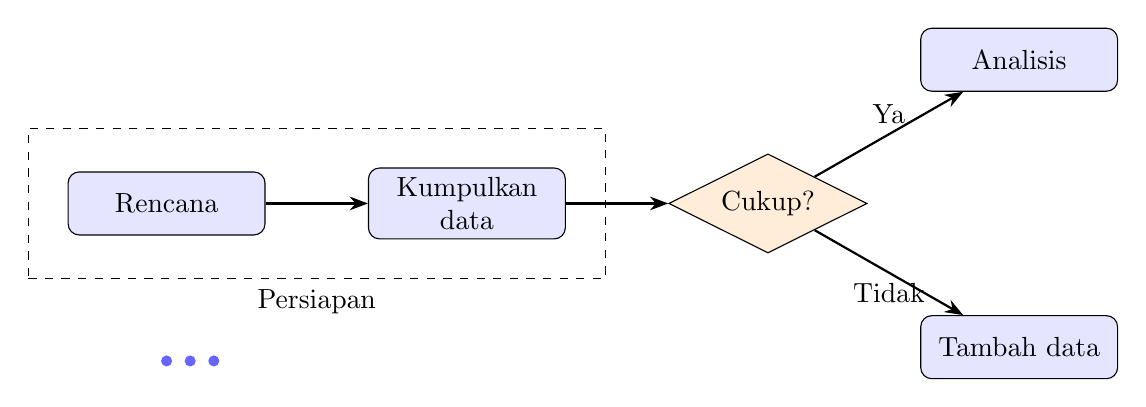
\begin{tikzpicture}[node distance=1.1cm and 1.3cm]
\node[tahap] (rencana) {Rencana};
\node[tahap,right=of rencana] (kumpul) {Kumpulkan\\data};
\node[keputusan,right=of kumpul] (cek) {Cukup?};
\node[tahap,above right=of cek] (analisis) {Analisis};
\node[tahap,below right=of cek] (ulang) {Tambah data};
\draw[relasi] (rencana) -- (kumpul);
\draw[relasi] (kumpul) -- (cek);
\draw[relasi] (cek) -- node[above] {Ya} (analisis);
\draw[relasi] (cek) -- node[below] {Tidak} (ulang);
\begin{scope}[on background layer]
\node[draw,dashed,inner sep=5mm,fit=(rencana)(kumpul),label=below:Persiapan] {};
\end{scope}
\foreach \x in {0,1,2} {\fill[blue!60] (\x*0.3,-2) circle (2pt);}
\end{tikzpicture}
\caption{Contoh alur penelitian bercabang.}
\end{figure}\end{document}
